\section{Attitude and Acceleration Autopilots}

The fourth stage used the course folder \texttt{6DOF - CURSO/03-autopiloto}. The professor's root-locus script was copied and adapted for the antiship missile. The same support files remained in the workflow:

\begin{itemize}
    \item \texttt{FTransDin.m};
    \item \texttt{calcula\_coef.m};
    \item \texttt{DadosControle.m};
    \item \texttt{Autopiloto.slx}.
\end{itemize}

The missile data, CG/inertia and aerodynamic matrix were replaced by the antiship missile data from the previous stage.

\subsection{Autopilot Architecture}

The attitude autopilot uses an inner \(q\)-feedback loop and an outer attitude loop:

\[
    \theta_c \rightarrow K_\theta \rightarrow
    \left(K_q,~\text{actuator},~q/\delta\right)
    \rightarrow \frac{1}{s} \rightarrow \theta.
\]

The acceleration autopilot uses the same inner \(q\)-feedback loop and an outer acceleration loop with an integrator:

\[
    A_{z,c} \rightarrow \frac{K_a}{s} \rightarrow
    \left(K_q,~\text{actuator},~q/\delta\right)
    \rightarrow A_z/\delta \rightarrow A_z.
\]

\subsection{Gain Schedule}

\begin{table}[H]
\centering
\caption{Computed autopilot gain schedule.}
\begin{tabular}{rrrrrr}
\toprule
\(t\) (s) & \(X_{CG}\) (m) & \(K_q\) attitude & \(K_\theta\) & \(K_q\) accel. & \(K_a\) \\
\midrule
0.000 & 2.8325 & 0.6000 & 9.3333 & 0.6000 & 0.0250 \\
1.725 & 2.8934 & 0.6667 & 10.6667 & 0.6667 & 0.0250 \\
3.450 & 2.9647 & 0.7333 & 12.0000 & 0.7333 & 0.0250 \\
115.350 & 2.6012 & 0.3333 & 8.0000 & 0.3333 & 0.0250 \\
\bottomrule
\end{tabular}
\end{table}

\begin{figure}[H]
\centering

\includegraphics[width=0.92\textwidth]{figures/gain_curves_vs_cg.png}
\caption{Internal and external gains as a function of CG.}
\end{figure}

\begin{figure}[H]
\centering

\includegraphics[width=0.9\textwidth]{figures/gain_schedule_vs_time.png}
\caption{Autopilot gain schedule along representative burn points.}
\end{figure}

\subsection{Root Locus and Step Responses}

\begin{figure}[H]
\centering

\includegraphics[width=0.75\textwidth]{figures/root_locus_inner_attitude.png}
\caption{Root locus of the common internal \(q\)-feedback loop.}
\end{figure}

\begin{figure}[H]
\centering

\includegraphics[width=0.75\textwidth]{figures/root_locus_outer_acceleration.png}
\caption{Root locus of the external acceleration loop.}
\end{figure}

\begin{figure}[H]
\centering

\includegraphics[width=0.84\textwidth]{figures/step_attitude.png}
\caption{Attitude autopilot unit-step response.}
\end{figure}

\begin{figure}[H]
\centering

\includegraphics[width=0.84\textwidth]{figures/step_acceleration_5g.png}
\caption{Acceleration autopilot response to a \(5g\) command.}
\end{figure}

\begin{table}[H]
\centering
\caption{Nominal requirement check.}
\begin{tabular}{lccc}
\toprule
Requirement & Result & Limit & Status \\
\midrule
Lateral acceleration capability & \(13.52g\) & \(\geq 5g\) & Satisfied \\
Attitude autopilot bandwidth & \(1.652~\text{Hz}\) & \(\geq 0.5~\text{Hz}\) & Satisfied \\
Acceleration autopilot bandwidth & \(0.537~\text{Hz}\) & \(\geq 0.5~\text{Hz}\) & Satisfied \\
\bottomrule
\end{tabular}
\end{table}

The acceleration loop was the limiting case. The initial root-locus gain was too aggressive for the nominal model, so the external gain was adjusted to \(K_a=0.025\). This kept the loop stable while maintaining bandwidth above \(0.5~\text{Hz}\).

\subsection{Engagement Check With Autopilot Constraints}

The final check connects the autopilot limits to the mission geometry. A horizontal point-mass engagement was run with Mach \(0.9\) at \(10~\text{m}\), \(5g\) lateral acceleration saturation, seeker cone of \(40^\circ\), and an airframe response of \(w_n=0.5~\text{Hz}\). Terminal guidance used proportional navigation. Case 1 switched to terminal guidance at \(20~\text{km}\); Case 2 first used a pre-programmed turn until the target entered the seeker cone.

\begin{table}[H]
\centering
\caption{Engagement results using R4 constraints.}
\begin{tabular}{lccc}
\toprule
Case & Minimum range & Time & Status \\
\midrule
65 km, bearing \(0^\circ\) & \(48.93~\text{m}\) & \(212.10~\text{s}\) & Satisfied \\
15 km, bearing \(90^\circ\) & \(47.06~\text{m}\) & \(54.43~\text{s}\) & Satisfied \\
\bottomrule
\end{tabular}
\end{table}

\begin{figure}[H]
\centering
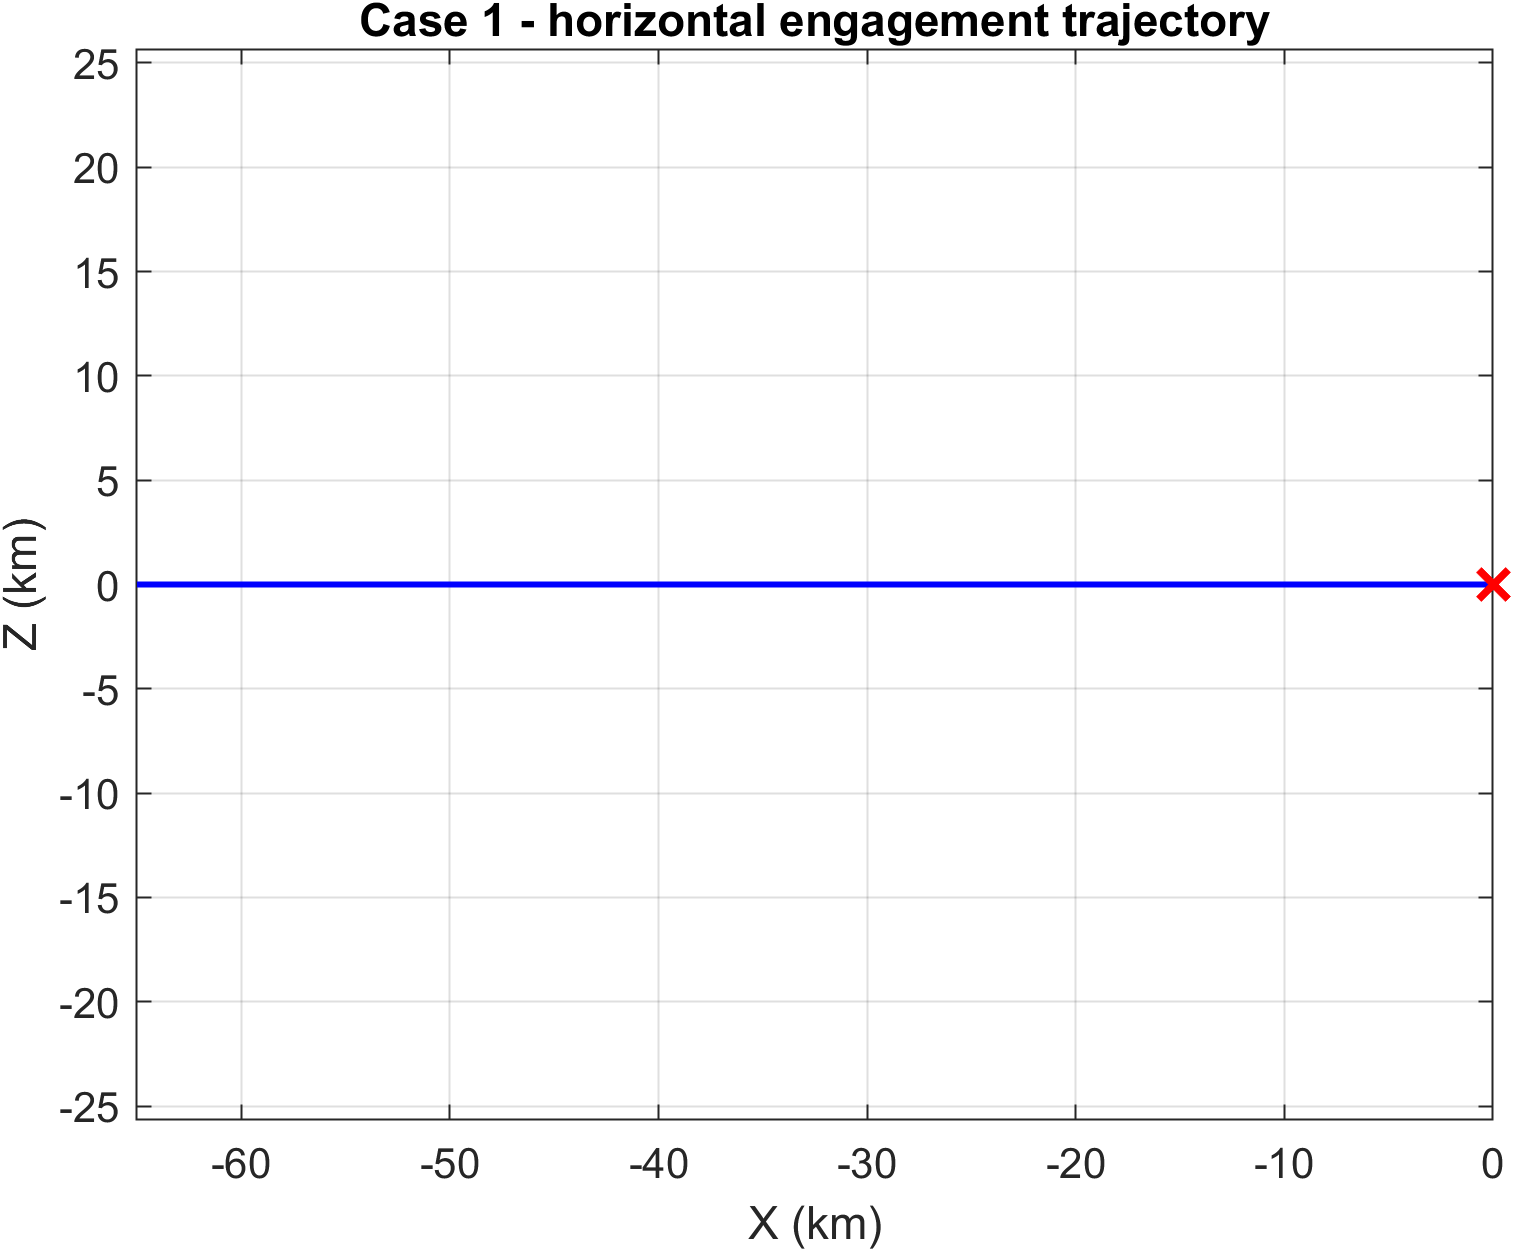
\includegraphics[width=0.78\textwidth]{figures/case1_engagement_trajectory.png}
\caption{Case 1 trajectory with R4 constraints.}
\end{figure}

\begin{figure}[H]
\centering
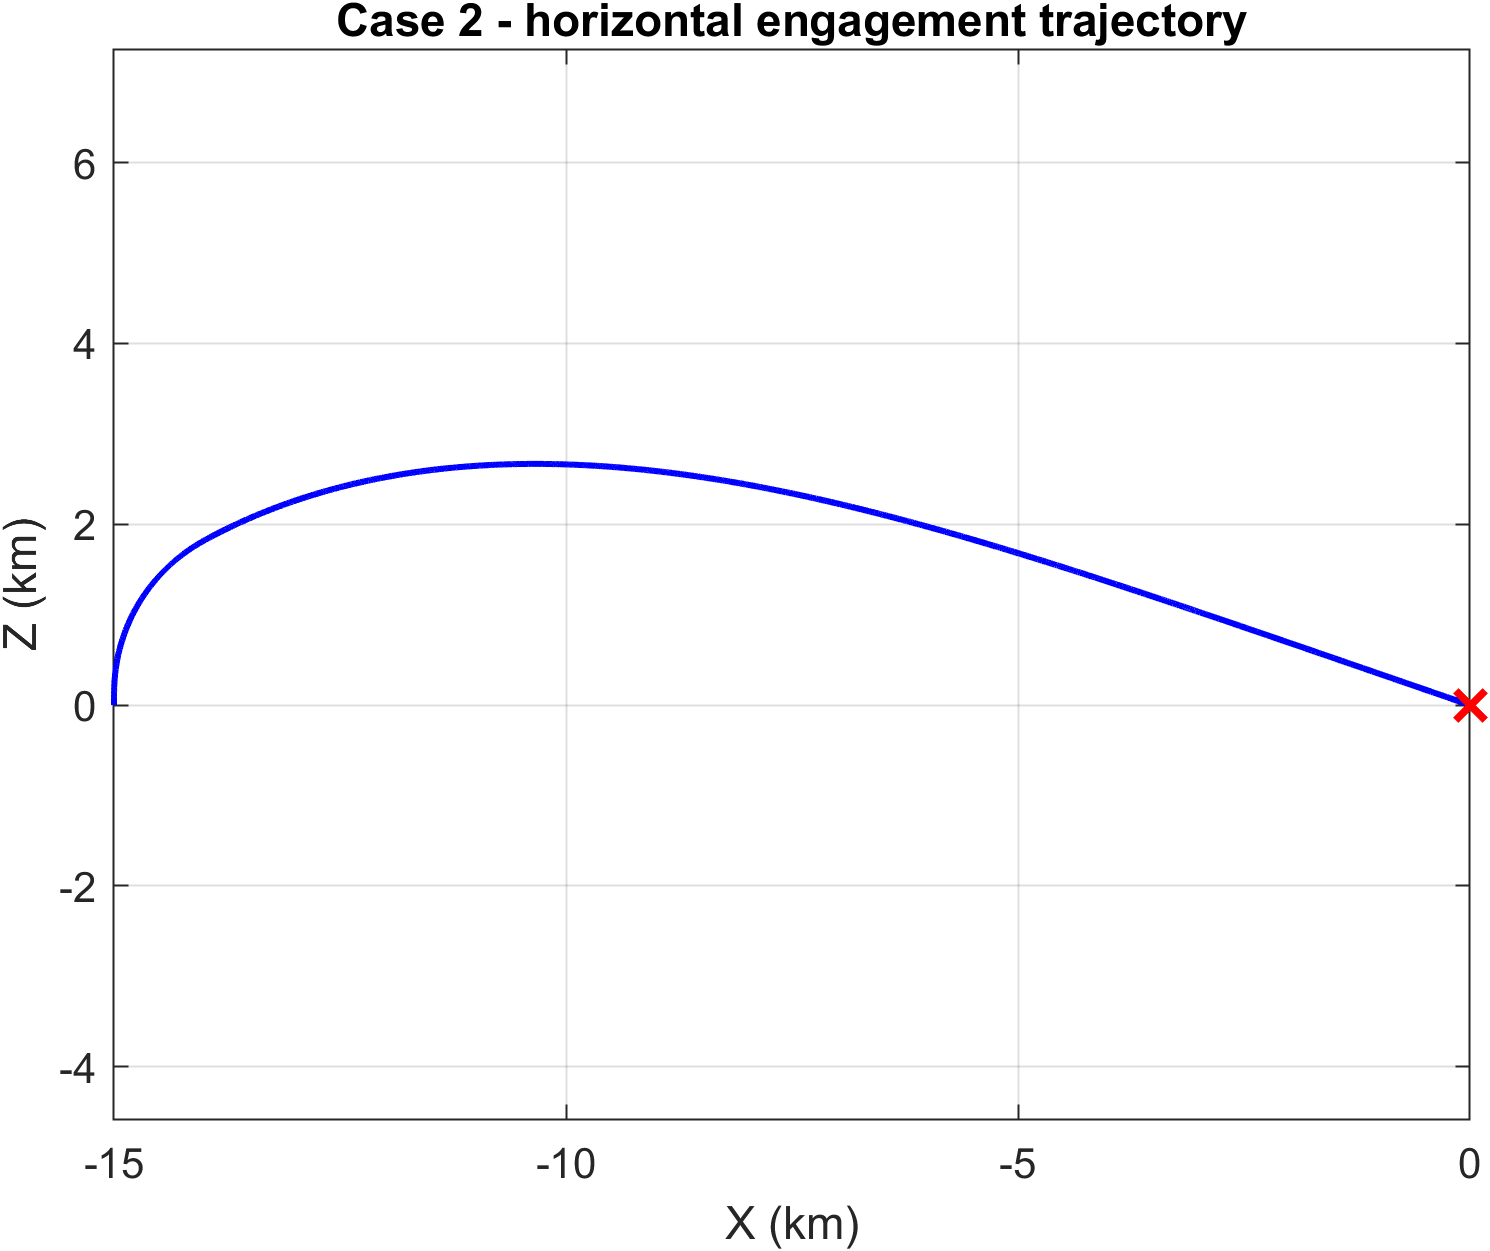
\includegraphics[width=0.78\textwidth]{figures/case2_engagement_trajectory.png}
\caption{Case 2 trajectory with R4 constraints.}
\end{figure}

Both engagement cases pass the \(50~\text{m}\) miss-distance criterion. The second case is the sizing case for maneuvering because it reaches the \(5g\) lateral acceleration limit during the initial turn.
